\subsection{Delay}
Delay is an audio effect which memorizes the input signal for a customized time, and then release it without changing it. The delayed signal can either be played back multiple times or only once . When the signal is delayed and then played back multiple times, it can either be amplified or attenuated. If the delayed signal is amplified, it will start to oscillate. If the wanted effect is an echo, the delayed signal shouldn't be kept alive, then the gain in the feedback must be reduced in order to attenuate the signal.  \autoref{fig:delay_block} shows a block diagram of a simple delay, "echo" unit.


\begin{figure} [htbp]
 \centering
\begin{picture}(0,0)%
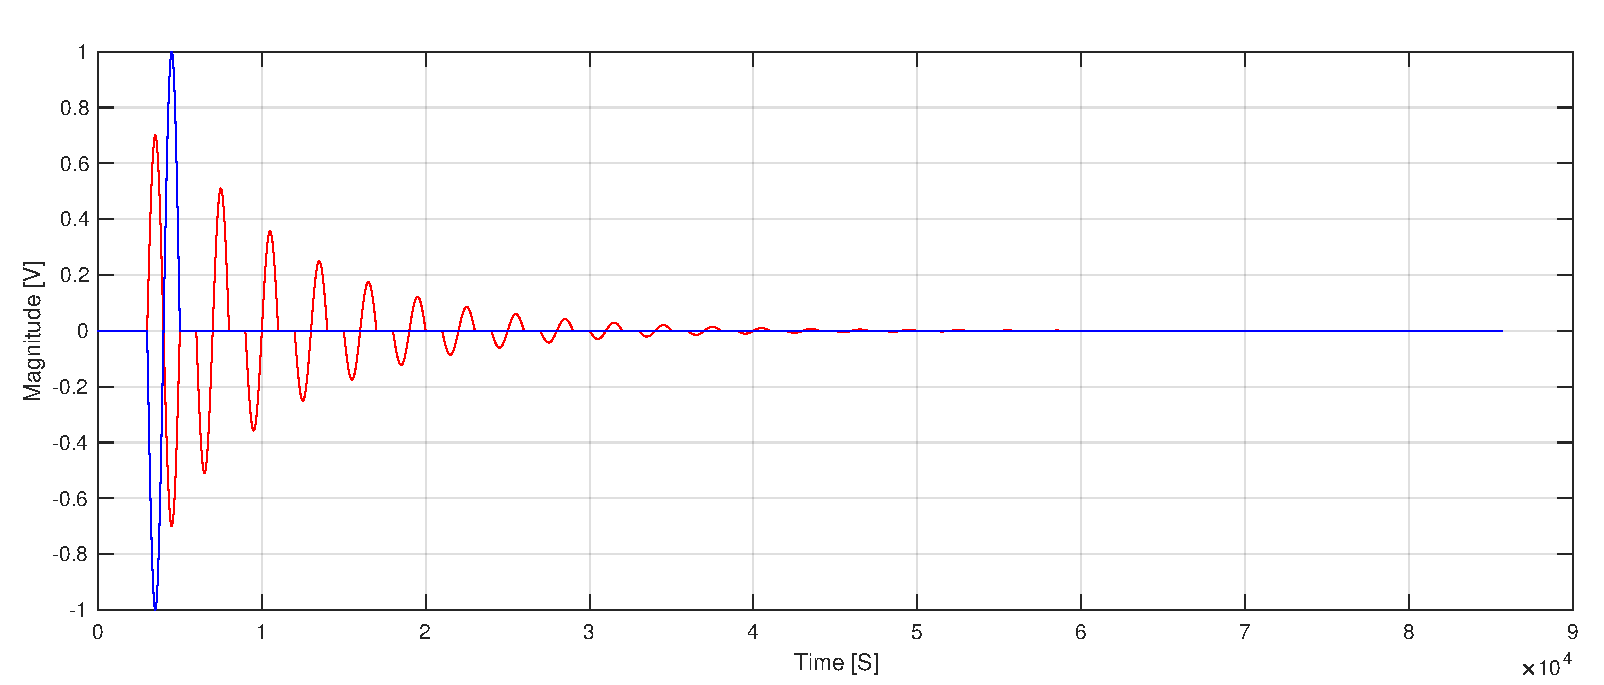
\includegraphics{delay.pdf}%
\end{picture}%
\setlength{\unitlength}{4144sp}%
%
\begingroup\makeatletter\ifx\SetFigFont\undefined%
\gdef\SetFigFont#1#2#3#4#5{%
  \reset@font\fontsize{#1}{#2pt}%
  \fontfamily{#3}\fontseries{#4}\fontshape{#5}%
  \selectfont}%
\fi\endgroup%
\begin{picture}(5035,1752)(1491,-118)
\put(1506,659){$Input$}%
\put(3106,479){$Delay$}%
\put(3736,1469){$Gain$}%
\put(5814,672){$Output$}%
\end{picture}%
  \caption{The photo shows a block diagram on a delay unit citep{delay_block}}
  \label{fig:delay_block}
\end{figure}

The block diagram \autoref{fig:delay_block} shows a delay unit with a feedback line that has an adjustable gain. The feedback signal is either attenuated or amplified depending on the gain value and then added to the delay line input. \cite{delay_echo} The following \autoref{fig:delay_echo} shows the effect in time domain.

\begin{figure} [htbp]
 \centering
  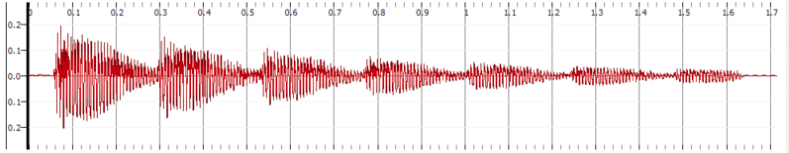
\includegraphics[width=1\textwidth]{delay_echo}
  \caption{The photo shows a echo in time domain}
  \label{fig:delay_echo}
\end{figure}

The \autoref{fig:delay_echo} shows that the main signal is repeated and attenuated 6 time before it is totally attenuated.